\section{Introduction}
  \IEEEPARstart{T}{his report} details the implementation of a pair of non-photorealistic
  rendering algorithms using OpenGL.  These rendering algorithms were then
  tested on a horse model to see their effectiveness.

  The first algorithm was based off what is known as ``\emph{three-tone
  shading},'' this is a technique primarily used for generating images that look
  like cartoon drawings.

  The second algorithm was an attempt at a ``\emph{pencil shading}'' algorithm.
  This involves rendering the 3D model as if it was hand shaded using a
  technique like cross-hatching.

  \subsection{Three-Tone shading}

    Figure \ref{cartoon} shows a real-life example of two-tone shading.  This is
    basically the same as flat-shading the image (drawing each section in a
    single constant colour) then adding in a darker shadow section to provide a
    sense of depth.  Three-tone shading takes this a step further and adds in a
    lighter highlight section that provides another clue for the depth sensing.

    The actual implementation of three-tone shading is relatively simple.  It is
    basically the diffuse term of the standard lighting model, restricted to
    just three tones for shadow, normal and highlights.

  \subsection{Pencil Shading}

    Figure \ref{shading} shows a variety of real-life pencil shading techniques.
    The main outcome of all these techniques is more graphite left on the darker
    areas, the different methods to achieve this result provide a different
    feeling for the images.  The main technique focused on for this
    implementation was cross-hatching, a better image of this can be seen in
    Figure \ref{hatching}.  The cross-hatching technique uses a large number of
    short line segments overlapping, the darker the region the more line
    segments are used.  This provides for an easy implementation by a real-time
    rendering algorithm, simply overlay more line segments on dark sections.

    The method chosen to implement the cross-hatching was composed of three
    major sections; first a texture had to be loaded to use as the basis of the
    line segments, next the model had to be pre-processed to extract data
    required for locating the texture on the segments, finally during run-time a
    few calculations had to be performed to get the correct darkness.

    To provide easy storage and access of the texture it was decided to use a 3D
    texture object.  This allowed the lines to be stored across the first and
    second dimensions and the differing darkness level to be stored up the third
    dimension.  This also provided very easy access in the shader hardware to
    acquire the texture value without any branching.

    \subsubsection{Texture Creation}
      
      The texture creation used was the weakest point of the pencil shading
      algorithm.  The implementation simply iterated down through the layers of
      the 3D texture, at each layer it added a few more lines to that layer and
      all below it.  The lines added were simply complete horizontal lines
      across the entire texture, an example of the output can be seen in Figure
      \ref{tex-example}.

      \begin{figure}
        \centering
        \subfloat[][Two-tone shading.]{
          
\includegraphics[width=0.3\textwidth]{images/cartoon}
          \label{cartoon}
        }

        \subfloat[][Pencil hatching. \cite{hatching-source}]{
          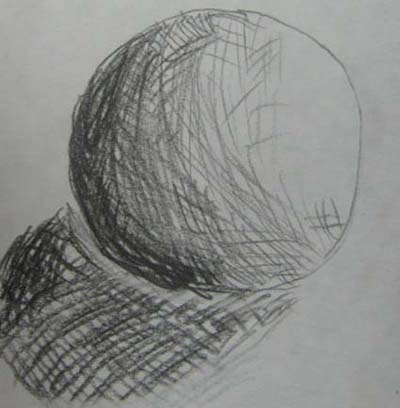
\includegraphics[width=0.3\textwidth]{images/hatching}
          \label{hatching}
        }

        \subfloat[][Different pencil shading techniques. \cite{shading-source}]{
          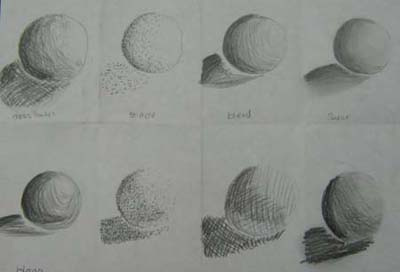
\includegraphics[width=0.4\textwidth]{images/shading}
          \label{shading}
        }

        \caption{Real-life examples of non-photorealistic renderings.}
      \end{figure}

      \begin{figure}
        \centering
        \subfloat[][n = 3]{
          
\includegraphics[width=0.22\textwidth]{images/tex-example3}
        }
        \subfloat[][n = 2]{
          
\includegraphics[width=0.22\textwidth]{images/tex-example2}
        }

        \subfloat[][n = 1]{
          
\includegraphics[width=0.22\textwidth]{images/tex-example1}
        }
        \subfloat[][n = 0]{
          
\includegraphics[width=0.22\textwidth]{images/tex-example0}
        }
        \caption{A small example texture (a black border has been added to the layers).}
        \label{tex-example}
      \end{figure}

    \subsubsection{Model Pre-processing}

      The model had to be pre-processed to identify where in the texture each
      vertex was.  Because the texture was generated with lines in a single
      direction the angle at which the texture was applied also had to be
      decided.  To best simulate real pencil strokes the angle to apply the
      texture was decided to be such that the lines align with the direction of
      maximum principal curvature ($T_1$ with associated curvature $\kappa_1$).
      Figure \ref{principal-curvature} shows how the two directions of principal
      curvature relate to the normal vector and tangent plane at a point, $T_1$
      is the vector lying within the tangent plane and the principal curvature
      plane with the maximum curvature value.

      \begin{figure}
        \centering
        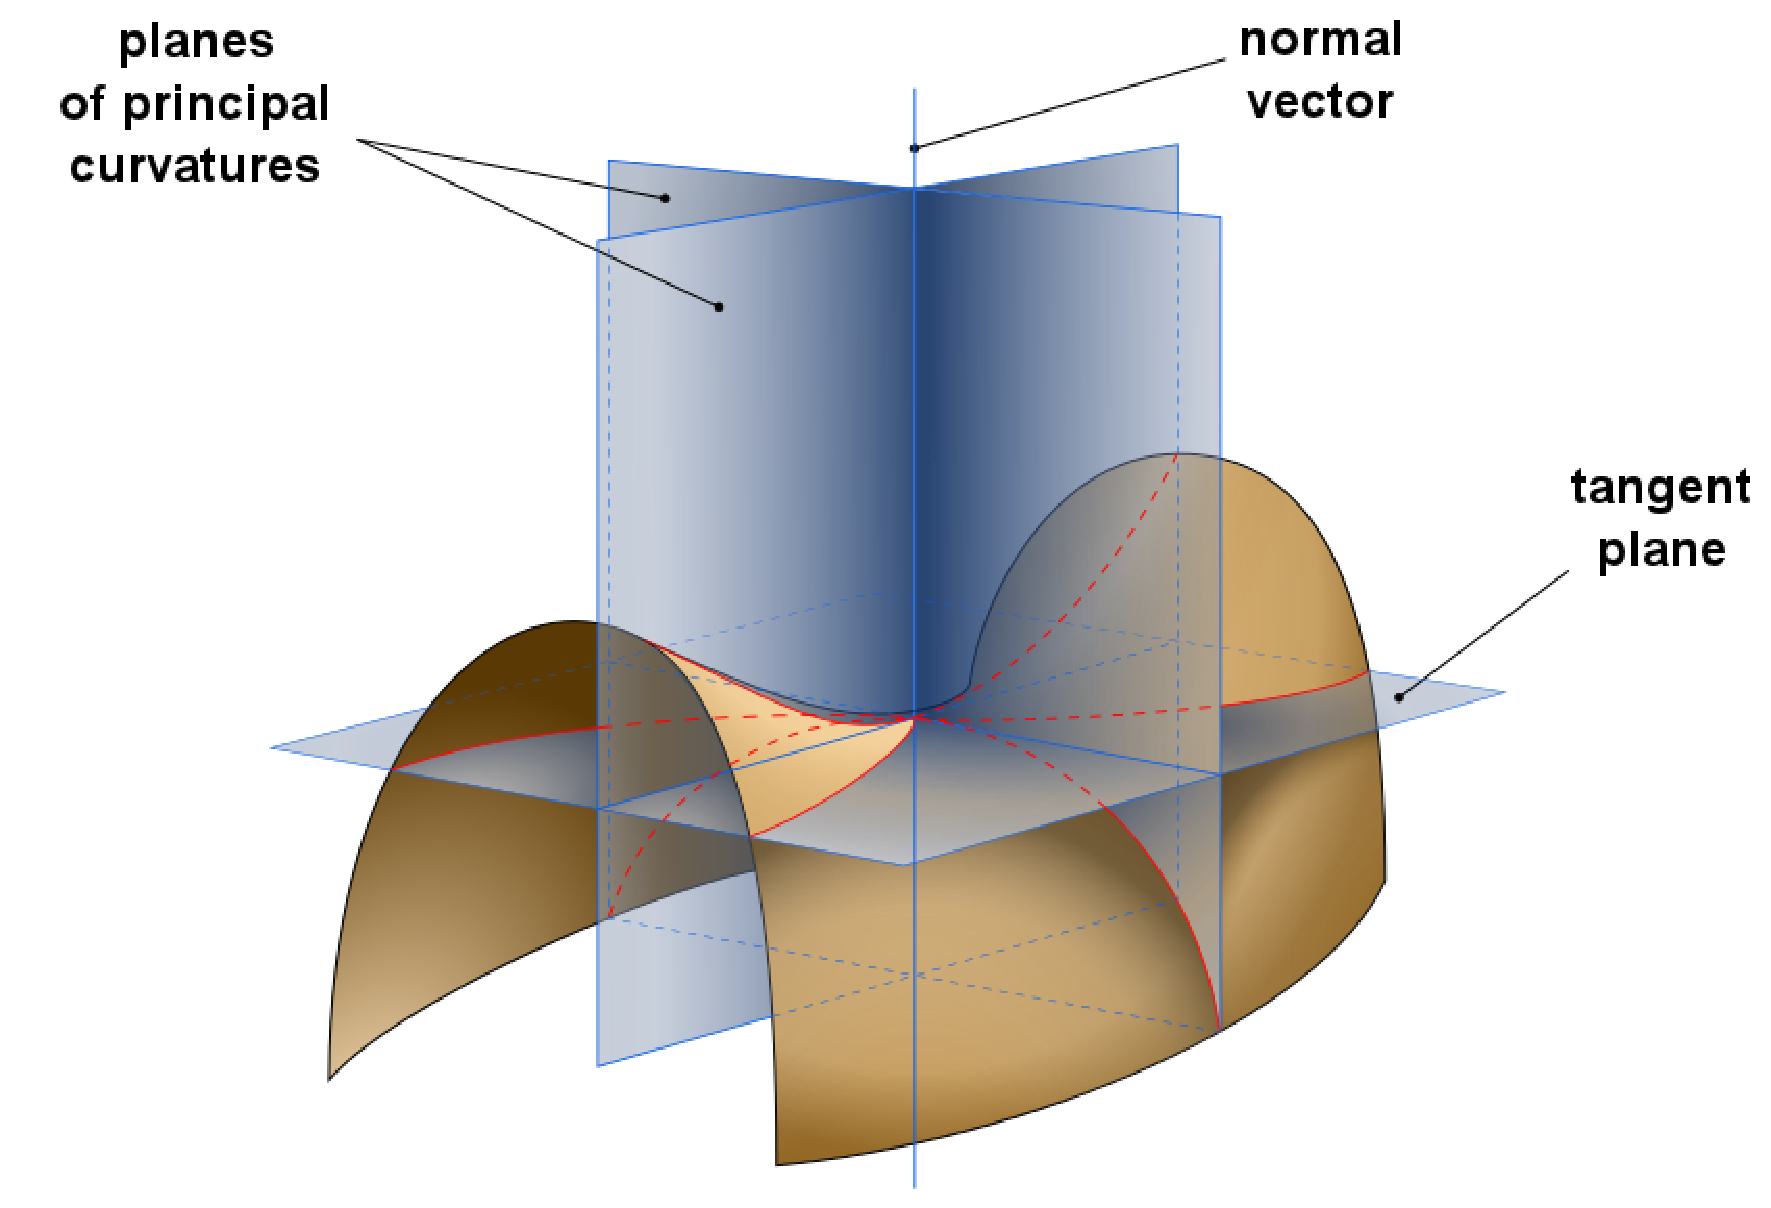
\includegraphics[width=0.45\textwidth]{images/principal-curvature}
        \caption{Saddle surface with normal planes in directions of principal
        curvatures. \cite{principal-curvature-source}}
        \label{principal-curvature}
      \end{figure}

      Obviously since most models passed to the program will not have a simple
      mathematical description this direction of maximum curvature will have to
      be approximated.  Timothy D. Gatzke and Cindy M. Grimm performed a large
      test of different methods of estimating principal curvature
      parameters\cite{curvature-study}.  From a quick reading of this the method
      proposed by Taubin\cite{taubin} was chosen.  While this is a relatively
      error prone method it has a very simple implementation; in this case
      errors do not matter overly as any real hand-drawn image would contain a
      multitude of errors anyway.

      The basic outline of the method is to take a variety of data points from
      the one-ring neighourhood of the vertex in question (mainly consisting of
      normal approximations at the points along with vectors from the point in
      question to each point), process this data to arrive at a 3x3 matrix with
      eigenvalues and eigenvectors obeying a fixed homogenous linear
      relationship with the required valeus.  This matrix can then be
      constrained to the tangent plane with a Householder transformation and the
      resulting 2x2 sub-matrix can easily be diagonalised with a Givens
      rotation.  Once the matrix has been diagonalised computing the eigenvalues
      and eigenvectors is simple and can be used to directly recover $\kappa_1$
      and $T_1$.

      Once these values are found the final step is to use these to relate each
      vertex $\left(x, y, z\right)$ to it's corresponding texture co-ordinate
      $\left(s, t\right)$.  Because the model is kept as a triangle mesh each
      face will have three $T_1$ values associated with it, one at each vertex.
      To provide a simulation of multiple crossing lines at different angles
      these are used to generate three different sets of texture co-ordinates
      for each face.

      To compute the $s$ and $t$ values one of the vertices is chosen to be the
      source vertex ($a$), this is given co-ordinates $\left(s, t\right) =
      \left(0.0, 0.0\right)$.  First the direction vectors to each of the other
      vertices ($v_{ab}$, $v_{ac}$) is projected on to the tangent plane at the
      source vertex using the normal ($n_a$):

      \begin{align}
        \bar{v_{ab}} &= v_{ab} - \left(v_{ab} \cdot n_a\right) n_a \\
        \bar{v_{ac}} &= v_{ac} - \left(v_{ac} \cdot n_a\right) n_a
      \end{align}

      These tangent direction vectors are then projected on to the directions of
      maximum and minimum principal curvature to determine their $s$ and $t$
      values:

      \begin{align}
        \left(s_b, t_b\right) &= \left(
          \bar{v_{ab}} \cdot T_1, \bar{v_{ab}} \cdot T_2
        \right) \\
        \left(s_c, t_c\right) &= \left(
          \bar{v_{ac}} \cdot T_1, \bar{v_{ac}} \cdot T_2
        \right)
      \end{align}

      This is then repeated with each of the vertices set as vertex $a$.  This
      results in 3 sets of texture co-ordinates for each vertex that are passed
      through to the shaders.

    \subsubsection{Run-time Processing}

      During run-time the only calculation that needs to be performed is
      determining the final texture value.  This is based off the diffuse term
      of the standard lighting model, ($p = \max\left(n \cdot l, 0.0\right)$
      where $n$ is the normal at the point and $l$ is the vector towards the
      light source).  Once this has been determined the 3D texture is simply
      accessed at $\left(s, t, p\right)$ with linear interpolation.
